% !TeX spellcheck = da_DK
%implementing document formatting:
\documentclass[a4paper,11pt,fleqn,dvipsnames,oneside,openright,oldfontcommands]{memoir} 	% Openright aabner kapitler paa hoejresider (openany begge)

\usepackage{xfrac}
\usepackage{booktabs}
\usepackage[table,xcdraw]{xcolor}

%%%%%%%%% Indsat random
%makes it possible to refer to the name of a chapter rather than just the number.
\usepackage{nameref}
\usepackage{pdfpages}
\usepackage{marvosym}
\usepackage{setspace}
\usepackage{graphicx} % For at sætte 2 billeder ved siden af hinanden

%package for writing program code in latex
\usepackage{listings}
%%%%%%%%%%%%%%%%%%%%%%

% ¤¤ Oversaettelse og tegnsaetning ¤¤ %
\usepackage[T1]{fontenc}					% Output-indkodning af tegnsaet (T1)
\usepackage[danish]{babel}					% Dokumentets sprog
\usepackage[utf8]{inputenc}					% Input-indkodning af tegnsaet (UTF8)
\usepackage{ragged2e,anyfontsize}			% Justering af elementer
\usepackage{fixltx2e}						% Retter forskellige fejl i LaTeX-kernen			
\usepackage{gensymb}						% Nu kan der skrices procent tegn med \degree				
				
																							
% ¤¤ Figurer og tabeller (floats) ¤¤ %
\usepackage{graphicx} 						% Haandtering af eksterne billeder (JPG, PNG, EPS, PDF)
%\usepackage{eso-pic}						% Tilfoej billedekommandoer paa hver side
\usepackage{wrapfig}						% Indsaettelse af figurer omsvoebt af tekst. \begin{wrapfigure}{Placering}{Stoerrelse}
\usepackage{multirow}                		% Fletning af raekker og kolonner (\multicolumn og \multirow)
\usepackage{multicol}         	        	% Muliggoer output i spalter
\usepackage{rotating}						% Rotation af tekst med \begin{sideways}...\end{sideways}
\usepackage{colortbl} 						% Farver i tabeller (fx \columncolor og \rowcolor)
\usepackage{xcolor}							% Definer farver med \definecolor. Se mere: http://en.wikibooks.org/wiki/LaTeX/Colors
\usepackage{flafter}						% Soerger for at floats ikke optraeder i teksten foer deres reference
\let\newfloat\relax 						% Justering mellem float-pakken og memoir
\usepackage{float}							% Muliggoer eksakt placering af floats, f.eks. \begin{figure}[H]
\usepackage{array,booktabs,xcolor,longtable} % kan lave \hdashline i tabellertabe
\usepackage{arydshln}
\usepackage{tabu}
\usepackage{epstopdf} 						% Muligoer brugen af eps filer i latex

	
	
% ¤¤ Matematik mm. ¤¤
\usepackage{amsmath , amsthm , amsfonts , amssymb, float, stmaryrd} 		% Avancerede matematik-udvidelser
%\usepackage{mathtools}						% Andre matematik- og tegnudvidelser
\usepackage{textcomp}                 		% Symbol-udvidelser (f.eks. promille-tegn med \textperthousand )
\usepackage{rsphrase}						% Kemi-pakke til RS-saetninger, f.eks. \rsphrase{R1}
\usepackage[version=3]{mhchem} 				% Kemi-pakke til flot og let notation af formler, f.eks. \ce{Fe2O3}
\usepackage{siunitx}						% Flot og konsistent praesentation af tal og enheder med \si{enhed} og \SI{tal}{enhed}
\sisetup{output-decimal-marker = {,}}		% Opsaetning af \SI (DE for komma som decimalseparator) 

% ¤¤ Referencer og kilder ¤¤ %
\usepackage[danish]{varioref}				% Muliggoer bl.a. krydshenvisninger med sidetal (\vref)
\usepackage[numbers]{natbib}				% Udvidelse med naturvidenskabelige citationsmodeller
%%\usepackage[sort&compress,square,comma,numbers]{natbib}
\newcommand{\citer}[1]{\citeauthor{#1},~\citeyear{#1}~\cite{#1}}

%\DeclareRobustCommand{\citer}[1]{\citeauthor{#1},~\citeyear{#1}~\cite{#1}}
											% citere i teksten: "Et studie af 'forfatter', 'år' [kilde#] viser..."
%\usepackage{xr}							% Referencer til eksternt dokument med \externaldocument{<NAVN>}
%\usepackage{glossaries}					% Terminologi- eller symbolliste (se mere i Daleifs Latex-bog)
\usepackage{lastpage}					% Gør det mulig at refere til sidste side 

% ¤¤ Misc. ¤¤ %
\usepackage{listings}						% Placer kildekode i dokumentet med \begin{lstlisting}...\end{lstlisting}
\usepackage{lipsum}							% Dummy text \lipsum[..]
\usepackage[shortlabels]{enumitem}			% Muliggoer enkelt konfiguration af lister
\usepackage{pdfpages}						% Goer det muligt at inkludere pdf-dokumenter med kommandoen \includepdf[pages={x-y}]{fil.pdf}	
\pdfoptionpdfminorversion=6					% Muliggoer inkludering af pdf dokumenter, af version 1.6 og hoejere
\pretolerance=2500 							% Justering af afstand mellem ord (hoejt tal, mindre orddeling og mere luft mellem ord)


% Kommentarer og rettelser med \fxnote. Med 'final' i stedet for 'draft' udloeser hver note en error i den faerdige rapport.
\usepackage[footnote,final,danish,silent,nomargin]{fixme}		


%%%% CUSTOM SETTINGS %%%%

% ¤¤ Marginer ¤¤ %
\setlrmarginsandblock{3.0cm}{2.5cm}{*}		% \setlrmarginsandblock{Indbinding}{Kant}{Ratio}
\setulmarginsandblock{2.5cm}{3.0cm}{*}		% \setulmarginsandblock{Top}{Bund}{Ratio}
\checkandfixthelayout 						% Oversaetter vaerdier til brug for andre pakker

%	¤¤ Afsnitsformatering ¤¤ %
\setlength{\parindent}{0mm}           		% Stoerrelse af indryk
\setlength{\parskip}{3mm}          			% Afstand mellem afsnit ved brug af double Enter
\linespread{1,1}							% Linie afstand



% ¤¤ Indholdsfortegnelse ¤¤ %
\setsecnumdepth{subsection}		 			% Dybden af nummerede overkrifter (part/chapter/section/subsection)
\maxsecnumdepth{subsection}					% Dokumentklassens graense for nummereringsdybde
\settocdepth{section} 					% Dybden af indholdsfortegnelsen

% ¤¤ Lister ¤¤ %
\setlist{
  topsep=0pt,								% Vertikal afstand mellem tekst og listen
  itemsep=-1ex,								% Vertikal afstand mellem items
} 

%hyperlinks in the tabel of contents - comment this out before the report is printed.
\usepackage{hyperref}
\hypersetup{
	bookmarks = true,  % Show 'bookmark'-frame in pdf.
	colorlinks = true, % True = colored links, False = framed links.
	citecolor = black,  % Link color for references.
	linkcolor = black,  % Link color in table of contents.
	urlcolor = black,   % Link color for extern URLs.
}

% ¤¤ Opsaetning af figur- og tabeltekst ¤¤ %
\usepackage{caption}
\usepackage{subcaption}
\captionnamefont{\small\bfseries\itshape}	% Opsaetning af tekstdelen ('Figur' eller 'Tabel')
\captiontitlefont{\small}					% Opsaetning af nummerering
\captiondelim{. }							% Seperator mellem nummerering og figurtekst
\hangcaption								% Venstrejusterer flere-liniers figurtekst under hinanden
%\captionwidth{0.9\textwidth}					% Bredden af figurteksten
\setlength{\belowcaptionskip}{0pt}			% Afstand under figurteksten
\captionsetup[figure]{labelfont={bf,it},font={it}} % sætter nummer til fed og kursis. Resten til fed + skriften er mindre end resten
\captionsetup[table]{labelfont={bf,it},font={it}} 


% ¤¤ Opsaetning af listings ¤¤ %

\definecolor{commentGreen}{RGB}{34,139,24}
\definecolor{stringPurple}{RGB}{208,76,239}

\lstset{language=Matlab,					% Sprog
	basicstyle=\ttfamily\scriptsize,		% Opsaetning af teksten
	keywords={for,if,while,else,elseif,		% Noegleord at fremhaeve
			  end,break,return,case,
			  switch,function},
	keywordstyle=\color{blue},				% Opsaetning af noegleord
	commentstyle=\color{commentGreen},		% Opsaetning af kommentarer
	stringstyle=\color{stringPurple},		% Opsaetning af strenge
	showstringspaces=false,					% Mellemrum i strenge enten vist eller blanke
	numbers=left, numberstyle=\tiny,		% Linjenumre
	extendedchars=true, 					% Tillader specielle karakterer
	columns=flexible,						% Kolonnejustering
	breaklines, breakatwhitespace=true,		% Bryd lange linjer
}

% ¤¤ Navngivning ¤¤ %
\addto\captionsdanish{
	\renewcommand\appendixname{Appendiks}
	\renewcommand\contentsname{Indholdsfortegnelse}	
	\renewcommand\appendixpagename{Appendiks}
	\renewcommand\appendixtocname{Appendiks}
	\renewcommand\cftchaptername{\chaptername~}				% Skriver "Kapitel" foran kapitlerne i indholdsfortegnelsen
	\renewcommand\cftappendixname{\appendixname~}			% Skriver "Appendiks" foran appendiks i indholdsfortegnelsen
}

% ¤¤ Kapiteludssende ¤¤ %
\definecolor{numbercolor}{gray}{0.7}		% Definerer en farve til brug til kapiteludseende
\newif\ifchapternonum

\makechapterstyle{jenor}{					% Definerer kapiteludseende frem til ...
	\renewcommand\beforechapskip{0pt}
	\renewcommand\printchaptername{}
	\renewcommand\printchapternum{}
	\renewcommand\printchapternonum{\chapternonumtrue}
	\renewcommand\chaptitlefont{\fontfamily{pbk}\fontseries{db}\fontshape{n}\fontsize{20}{35}\selectfont\raggedright}
	\renewcommand\chapnumfont{\fontfamily{pbk}\fontseries{m}\fontshape{n}\fontsize{0.35in}{0in}\selectfont\color{black}}
	\renewcommand\printchaptertitle[1]{%
		\noindent
		\ifchapternonum
		\begin{tabularx}{\textwidth}{X}
			{\let\\\newline\chaptitlefont ##1\par} 
		\end{tabularx}
		\par\vskip-2.5mm\hrule
		\else
		\begin{tabularx}{\textwidth}{Xl}
			{\parbox[b]{\linewidth}{\chaptitlefont ##1}} & \raisebox{-5pt}{\chapnumfont \thechapter}
		\end{tabularx}
		\par\vskip2mm\hrule
		\fi
	}
}											% ... her

\chapterstyle{jenor}						% Valg af kapiteludseende - Google 'memoir chapter styles' for alternativer

% ¤¤ Sidehoved ¤¤ %

\makepagestyle{AAU}							% Definerer sidehoved og sidefod udseende frem til ...
\makepsmarks{AAU}{%
	\createmark{chapter}{left}{shownumber}{}{. \ }
	\createmark{section}{right}{shownumber}{}{. \ }
	\createplainmark{toc}{both}{\contentsname}
	\createplainmark{lof}{both}{\listfigurename}
	\createplainmark{lot}{both}{\listtablename}
	\createplainmark{bib}{both}{\bibname}
	\createplainmark{index}{both}{\indexname}
	\createplainmark{glossary}{both}{\glossaryname}
}
\nouppercaseheads											% Ingen Caps oenskes

\makeevenhead{AAU}{Gruppe 5406}{}{\leftmark}				% Definerer lige siders sidehoved (\makeevenhead{Navn}{Venstre}{Center}{Hoejre})
\makeoddhead{AAU}{\rightmark}{}{Aalborg Universitet}		% Definerer ulige siders sidehoved (\makeoddhead{Navn}{Venstre}{Center}{Hoejre})
\makeevenfoot{AAU}{\thepage}{}{}							% Definerer lige siders sidefod (\makeevenfoot{Navn}{Venstre}{Center}{Hoejre})
\makeoddfoot{AAU}{}{}{\thepage}								% Definerer ulige siders sidefod (\makeoddfoot{Navn}{Venstre}{Center}{Hoejre})
\makeheadrule{AAU}{\textwidth}{0.5pt}						% Tilfoejer en streg under sidehovedets indhold
\makefootrule{AAU}{\textwidth}{0.5pt}{1mm}					% Tilfoejer en streg under sidefodens indhold

\copypagestyle{AAUchap}{AAU}								% Sidehoved for kapitelsider defineres som standardsider, men med blank sidehoved
\makeoddhead{AAUchap}{}{}{}
\makeevenhead{AAUchap}{}{}{}
\makeheadrule{AAUchap}{\textwidth}{0pt}
\aliaspagestyle{chapter}{AAUchap}							% Den ny style vaelges til at gaelde for chapters
% ... her

\pagestyle{AAU}												% Valg af sidehoved og sidefod


%%%% CUSTOM COMMANDS %%%%

% ¤¤ Billede hack ¤¤ %
\newcommand{\figur}[4]{
		\begin{figure}[H] \centering
			\includegraphics[width=#1\textwidth]{billeder/#2}
			\caption{#3}\label{#4}
		\end{figure} 
}

% ¤¤ Specielle tegn ¤¤ %
\newcommand{\decC}{^{\circ}\text{C}}
\newcommand{\dec}{^{\circ}}
\newcommand{\m}{\cdot}


%%%% ORDDELING %%%%

\hyphenation{}

%%%%Fra engelsk til dansk i \autoref{•} %%%%
\renewcommand{\figureautorefname}{Figur}
\renewcommand{\sectionautorefname}{Afsnit}
\renewcommand{\subsectionautorefname}{Afsnit}
\renewcommand{\subsubsectionautorefname}{Afsnit}
\renewcommand{\tableautorefname}{Tabel}
\renewcommand{\appendixautorefname}{Appendiks}
\renewcommand{\equationautorefname}{Ligning}
\renewcommand{\itemautorefname}{Punkt}
\renewcommand{\chapterautorefname}{Kapitel}
\raggedbottom
%Figure references:
\newcommand{\figref}[1]{figur~\ref{#1}}

%Figure references after full stop/period:
\newcommand{\Figref}[1]{Figur~\ref{#1}}

%Table references:
\newcommand{\tabref}[1]{tabel~\ref{#1}}

%Table references after full stop/period:
\newcommand{\Tabref}[1]{Tabel~\ref{#1}}

%Appendix references:
\newcommand{\appref}[1]{appendiks~\ref{#1}}

%Appendix references after full stop/period:
\newcommand{\Appref}[1]{Appendiks~\ref{#1}}

%Section references:
\newcommand{\secref}[1]{afsnit~\ref{#1}}

%Section references:
\newcommand{\Secref}[1]{Afsnit~\ref{#1}}

%chapter references: 
\newcommand{\chapref}[1]{kapitel~\ref{#1}}

%chapter references: 
\newcommand{\Chapref}[1]{Kapitel~\ref{#1}}


%Units:
%inserting '\omit' before '{\put' prior ot final compile will fix allignment (and generate errors)
\newcommand{\unit}[1]{{\put(300,0){$\hfill\left[\: #1 \:\right]$}}}

%Text:
\newcommand{\tx}[1]{\text{#1}}

%Equation references:
%1 equation:
\renewcommand{\eqref}[1]{ligning~(\ref{#1})}
%2 equations:
\newcommand{\eqrefTwo}[2]{ligning~(\ref{#1}) og (\ref{#2})}
%3 equations:
\newcommand{\eqrefThree}[3]{ligning~(\ref{#1}), (\ref{#2}) og (\ref{#3})}
%4 equations:
\newcommand{\eqrefFour}[4]{ligning (\ref{#1}), (\ref{#2}), (\ref{#3}) og (\ref{#4})}
%5 equations:
\newcommand{\eqrefFive}[5]{ligning (\ref{#1}), (\ref{#2}), (\ref{#3}), (\ref{#4}) og (\ref{#5})}


%Equation references after full stop/period:
%1 equation:
\newcommand{\Eqref}[1]{Ligning~(\ref{#1})}
%2 equations:
\newcommand{\EqrefTwo}[2]{Ligning~(\ref{#1}) og (\ref{#2})}
%3 equations:
\newcommand{\EqrefThree}[3]{Ligning~(\ref{#1}), (\ref{#2}) og (\ref{#3})}
%4 equations:
\newcommand{\EqrefFour}[4]{Ligning (\ref{#1}), (\ref{#2}), (\ref{#3}) og (\ref{#4})}
%5 equations:
\newcommand{\EqrefFive}[5]{Ligning (\ref{#1}), (\ref{#2}), (\ref{#3}), (\ref{#4}) og (\ref{#5})}
\begin{document}

%numbers the pages with Roman numeral - starts from "i":
\frontmatter
\clearpage
\thispagestyle{empty}

%\begin{figure}[H]
%	\raggedleft
%		
\includegraphics[width=0.2\textwidth]{figures/aaulogo-da.png}
%\end{figure}


%\vspace*{\fill} 
%\begin{center}	
%	\begin{Huge}
%		P3 Projektrapport - efterår 2015\\
%		\vspace{5 mm}
%		\textbf{System til detektering af kropsbalance}\\
%		\vspace{3 mm}
%		Gruppe 375
%	\end{Huge}
%\end{center}
%\vspace*{\fill}

\begin{center}
	\vspace*{\baselineskip}
	\rule{\textwidth}{1.6pt}\vspace*{-\baselineskip}\vspace*{2pt} % Thick horizontal line
	\rule{\textwidth}{0.4pt}\\[\baselineskip] % Thin horizontal line
	
	{\huge Aktivitetsmåler til forebyggelse\\\hspace*{2ex} af fysisk inaktivitet hos børn \\[0.5\baselineskip] \large Projektrapport 4. semester}\\[0.2\baselineskip] % Title
	
	\rule{\textwidth}{0.4pt}\vspace*{-\baselineskip}\vspace{3.2pt} % Thin horizontal line
	\rule{\textwidth}{1.6pt}\\[\baselineskip] % Thick horizontal line
	\vspace*{5\baselineskip}
	\begin{figure}[H]
		\centering
		\begin{minipage}[c]{1\textwidth}
			
\includegraphics[width=.75\textwidth]{figures/forside2.PNG}
		\end{minipage}
		\hfill
	\end{figure}
	\vspace*{\fill}
	\scshape % Small caps
	{\Large Gruppe 4403\par}
	
	\vspace*{.8\baselineskip} % Whitespace between location/year and editors
	
	Aalborg Universitet,  01/02/2016 - 27/05/2016 \par % Location and year
\end{center} % Center all text
%{\color{white}X \\ X \\ X \\}

%\begin{center}
%	\textit{Gruppemedlemmer:}\\
%	Cecilie Sophie Rosenkrantz Topp, Frederik Skou Nielsen \\
%	Josefine Dam Gade, Line Sofie Hald, Morten Skaarup Larsen
%\end{center}
\begin{center}
	\line(1,0){400}
\end{center}

\clearpage
\thispagestyle{empty}
{\color{white}Dette giver en tom side}
\clearpage

%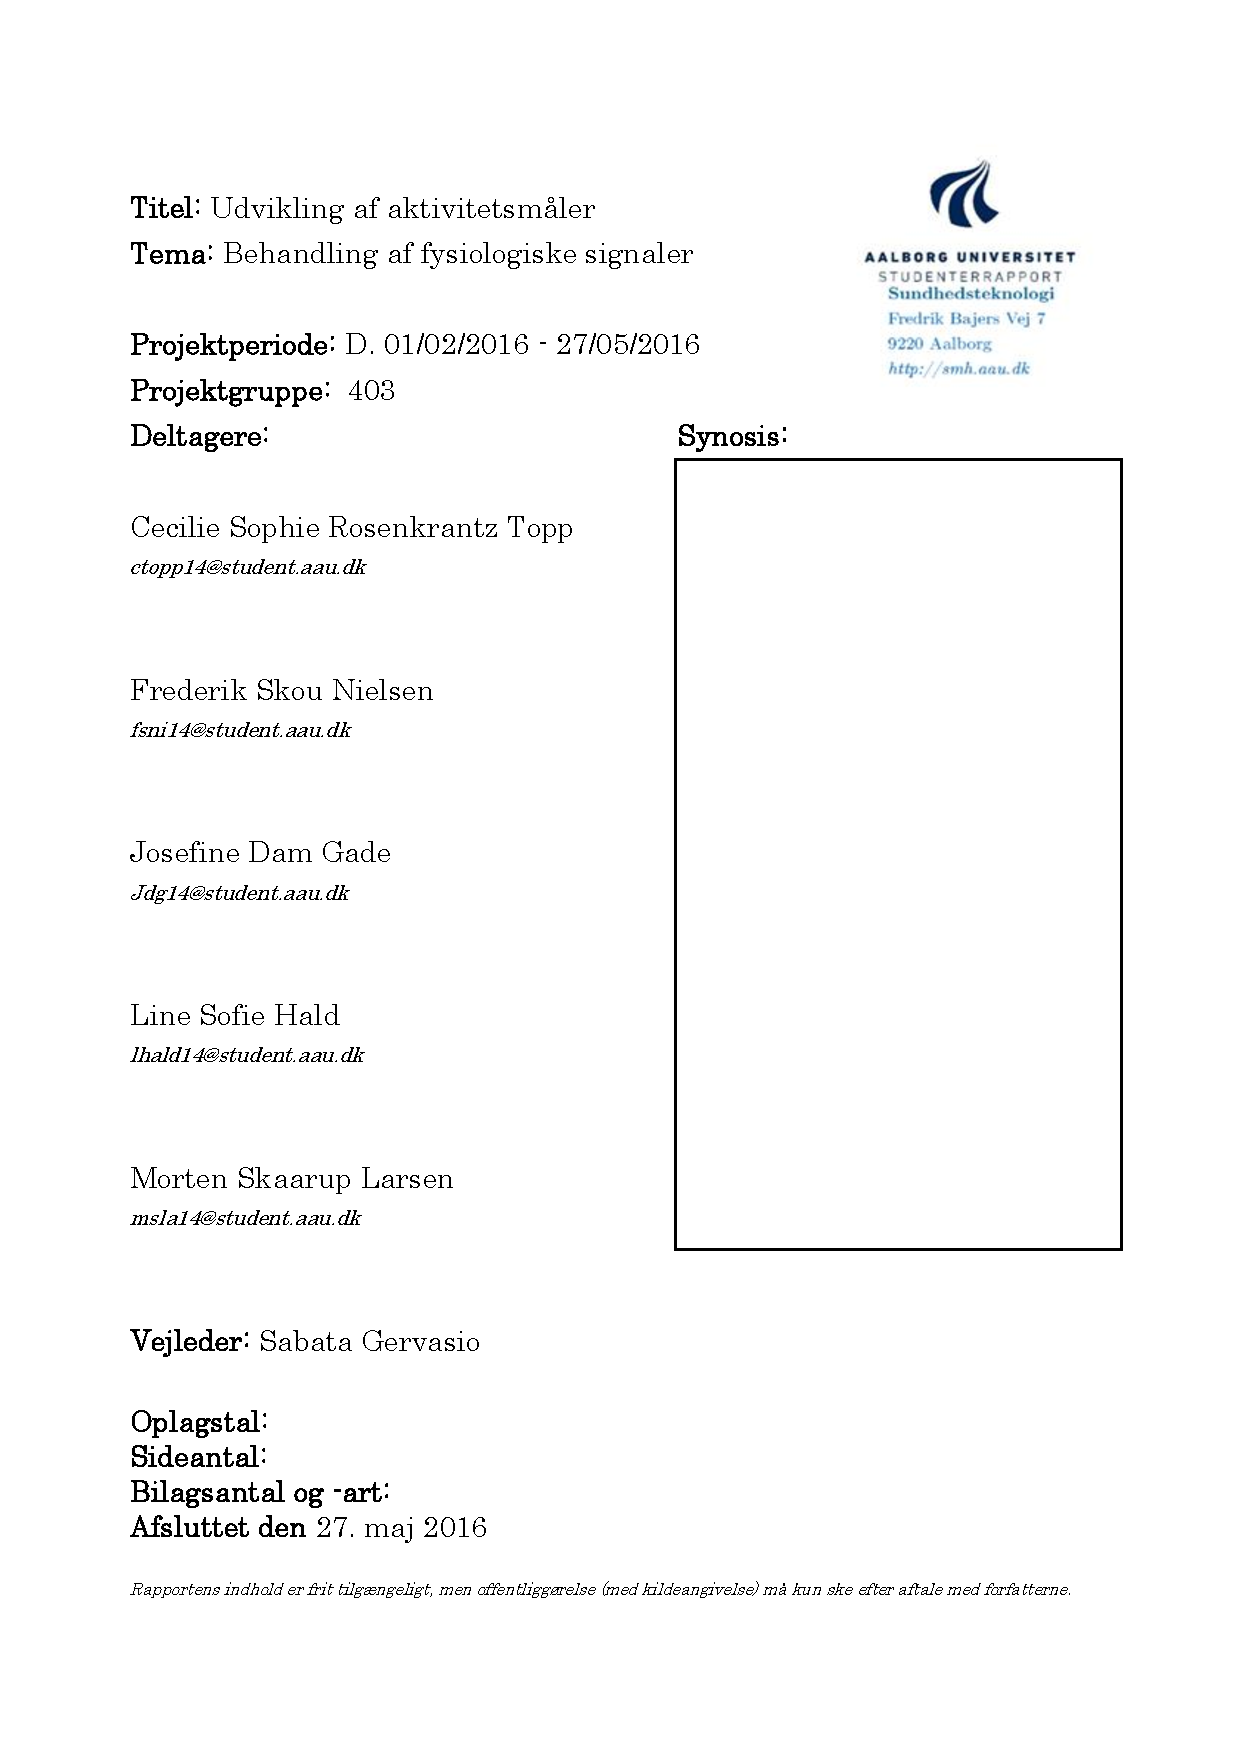
\includepdf[pages={1}]{rapportAfsnit/pFormaliteter/synopsis.pdf} \clearpage 
\include{rapportAfsnit/pFormaliteter/titelblad}
\chapter*{Forord og læsevejledning}\vspace{-.75cm}
% !TeX spellcheck = da_DK
\section*{Forord}
Denne rapport er udarbejdet som et 4. semesters projekt på bacheloruddannelsen i Sundhedsteknologi på Aalborg Universitet. Projektetperioden forløb fra 1. februar 2016 til 27. maj 2016. \\
Projektet tager udgangspunkt i studieordningen for bacheloruddannelsen i Sundhedsteknologi. Semesterets fokusområde er 'Behandling af fysiologiske signaler', hvor dette projekt tager udgangspunkt i projektforslaget 'Udvikling af aktivitetsmåler'. Formålet er blandt andet design, implementering og test af en prototype, der kan detektere fysisk aktivitet. Protoypen udvikles med henblik på at bestemme det fysiske aktivitetsniveau for børn i aldersgruppen 9-12 år. %Prototypen vil derfor involvere en dataopsamling fra analoge komponenter i form af et et accelerometer, et gyroskop og en pulssensor. Ydermere vil prototypen indeholde signal- og databehandling som muligøre digital visualisering på et grafisk brugerinterface.

%Projektet henvender sig til studerende på samme niveau eller andre interessere med et kendskab til basal analog og digital databehandling. \\
Der rettes en tak til vejleder Sabata Gervasio for et godt og lærerigt samarbejde under udarbejdelsen af denne rapport. Yderligere rettes der en tak til semesterkoordinater, John Hansen, for råd og vejledning til forståelse af semesterets nye mikrokontroller. 

\section*{Læsevejledning}
Projektet er opbygget af fem kapitler, en litteraturoversigt samt to bilag. Hvert kapitel og hovedafsnit indledes med et kursiv afsnit, som har til formål at vejlede læseren i henholdsvis kapitlets og hovedafsnittets indhold og sammenhæng i rapportens helhed.\\
Første kapitel består af en indledning og initierende problemstilling. Herefter er problemanalysen, der bearbejder den initierende problemstilling, hvilket leder frem til en problemformulering. Det tredje kapitel er problemløsning, hvori løsningsstrategi og essentielle teoretiske elementer beskrives. Yderligere indeholder kapitlet krav til prototypen og dets delelementer. Det efterfølgende kapitel består af design, implementering og test af systemets delementer samt en test af det samlede system. Afslutningsvis findes syntesen, indeholdende diskussion, konklusion og perspektivering.

Rapporten benytter Vancouver metoden til kildehenvisning. Alle benyttede kilder er at finde på side 91, hvor de er listet i numerisk rækkefølge. I tilfælde, hvor kilden befinder sig inden for punktum, tilhører denne kildehenvisning indholdet i den pågældende sætning. Er kildehenvisningen placeret efter punktummet i sætningen, tilhører kilden indholdet i det foregående afsnit. \\
Tabeller og figurer er nummereret efter deres respektive afsnit, hvorfor eksempelvis figur 1.1 er den første figur i kapitel 1.

Rapporten benytter forkortelser, hvor ordet skrives ud første gang det præsenteres med tilhørende forkortelse i parentes efter ordet. Efterfølgende vil denne forkortelse blive benyttet i resten af rapporten med undtagelse af overskrifter. 
\newpage

%the '*' allows the tableofcontents be excepted from the actual table of contents.
\tableofcontents* 

%numbers the pages with Arabic numeral - starts from 1.
\mainmatter


\chapter{......}\vspace{-.75cm}
%\input{rapportAfsnit/../..}
\cleardoublepage
\chapter{Syntese}\vspace{-.75cm}
%\input{rapportAfsnit/../..}

\begingroup
\label{litteraturliste}
\raggedright
\bibliographystyle{unsrtnat}
\bibliography{kilder}
\endgroup
\begin{appendices}
%	\input{rapportAfsnit/qBilag/pilotforsoeg}
%	\input{rapportAfsnit/qBilag/MCU}
\end{appendices}

\end{document}